\label{ch:problema}
\chapter{Descripción del problema}

En Android, por defecto, el desarrollador no cuenta con mecanismos para
definir políticas de confidencialidad e integridad que regulen
el flujo de información de sus aplicaciones. Siendo complejo prevenir fugas de
información del usuario, puesto que, el desarrollador carece de herramientas que
le garanticen la ausencia de flujos indeseados.\newline
Precisamente, una de las principales preocupaciones de seguridad en aplicativos
Android, es la manipulación de información del usuario.
Así lo evidencia un
estudio reciente de seguridad en dispositivos móviles, publicado por
McAfee\cite{McAfeeReport}, este señala  que una importante cantidad de
aplicaciones Android invaden la privacidad del usuario, reuniendo información
detallada de su desplazamiento, acciones en el dispositivo, y su vida personal.
De este modo, 80\% reúnen información de la ubicación, 82\%
hacen seguimiento de alguna acción en el dispositivo , 57\%
registran la forma de uso del celular (mediante Wi-Fi o
mediante la red de telefonía), y 36\% conocen información de
las cuentas de usuario.\newline
Las motivaciones para este tipo de acciones varían acorde al tipo de
información, por ejemplo: monitorear información de ubicación para mostrar
publicidad no solicitada; seguir las acciones sobre el dispositivo, para conocer
qué aplicaciones son rentables de desarrollar, o para ayudar a aplicaciones
maliciosas a evadir defensas; acceder a información de cuentas del usuario con
fines delictivos; obtener información de contactos y calendario
del usuario, buscando modificar los datos; obtener información del celular 
(número, estado, registro de MMS y SMS) para interceptar llamadas y enviar
mensajes sin consentimiento del usuario.\newline
Con o sin autorización de acceso, existen motivaciones suficientes para que un
tercero desee manipular información del usuario.\newline
Adicionalmente, el informe señala que una aplicación invasiva no necesariamente
contiene malware, y que su finalidad no siempre implica fraude; de las
aplicaciones que más vulneran la privacidad del usuario, 35\% contienen
malware.\newline 
Si bien, aplicaciones invasivas no necesariamente implican
malware y/o acciones delictivas, el cuestionamiento de fondo es la forma y
finalidad con que están accediendo la información, es decir, si información
de usuario manipulada por una determinada aplicación, realmente debería ser
accedida por otros aplicativos del dispositivo, aún cuando sean considerados no
maliciosos; y qué garantías puede ofrecer el desarrollador para que tal acceso,
efectivamente sea consentido.\newline 
La falta de control sobre los flujos de información de la aplicación puede
ocasionar fugas de información, generando problemas de seguridad tanto para
quien la implementa como para quien la usa.\newline
Como contramedida a este problema, la API de Android ofrece herramientas de
seguridad basadas en políticas de control de acceso, y el desarrollador puede
implementarlas en su aplicación. Sin embargo, estos mecanismos se centran en
regular el acceso de los usuarios del sistema a determinados recursos, y no en
verificar qué sucede con la información una vez es accedida.\newline 
Para superar tal carencia, diferentes trabajos de investigación han abordado el
problema de fuga de información en aplicaciones Android, tanto desde un enfoque
dinámico como desde un enfoque estático, la literatura existente al
respecto(TaintDroid\cite{TaintDroid}, Flow-Droid\cite{FlowDroid-Thesis},
DidFail\cite{DidFail}, DroidForce\cite{DroidForce}), indica que la mayoría de
propuestas hacen data-flow analysis mediante técnicas de análisis usando
tainting, partiendo del bytecode. Una característica sobresaliente entre estos
trabajos es el modelo de ataque, puesto que, se centran en analizar aplicaciones
de terceros asumiendo que el atacante provee bytecode malicioso. Guiar el
análisis de aplicaciones propias con el fin de verificar políticas de
confidencialidad e integridad, bajo tales propuestas, puede implicar: mayor
dificultad en el código a analizar, incompletitud en el análisis(under-tainting)
y no detección de flujos implícitos. Esto debido a que, aún cuando el
desarrollador conoce la funcionalidad de su propio código, las optimizaciones
realizadas por el compilador pueden adicionar complejidad al
mismo\cite[pag.~43]{SecureProgramming}; el seguimiento de los datos a través del
programa está centrado en datos marcados, datos no marcados quedan fuera del
análisis;   flujos de datos a través de estructuras de control, por ejemplo, las
sentencias if, permiten inferir valores de datos marcados como source, sin
necesidad de generar flujos explícitos entre sources y sinks, los cuales si
pueden ser detectados por las técnicas de análisis tainting.\newline Otra razón
fundamental para no  analizar aplicaciones propias con tales propuestas es que
están diseñadas para detectar flujos de datos indebidos, y no para garantizar el
cumplimiento de políticas de seguridad en una aplicación.\newline 
Los riesgos de seguridad tras el under-tainting de datos, y la ausencia de
garantías en el cumplimiento de determinadas políticas de seguridad, pueden
superarse mediante control de flujo de información, Information Flow
Control(IFC), puesto que, con esta técnica se analiza estáticamente la
aplicación para identificar todos los posibles caminos que podrían tomar sus
flujos de información, garantizando que a tiempo de ejecución, la
aplicación respeta políticas de seguridad.\newline

Finalmente, partiendo del contexto que se plantea, dónde se cuenta con el código
fuente Android, porque es el propio desarrollador quien requiere evaluar
políticas de confidencialidad en su aplicación, para  garantizarle
al usuario que la aplicación las cumple. Resulta apropiado proveer una
herramienta de apoyo al desarrollador, mediante la cual analice el flujo de
información de la aplicación próxima a liberar, y verifique el cumplimiento de
políticas de seguridad.
 
\section{Trabajos Relacionados}
\label{sec:trabajo}
\subsection{JIF}
\label{JIF-Tool}
JIF(Java Information Flow), es un lenguaje tipado de seguridad que
permite extender el lenguaje de programación Java,  con control de flujo de
información y control de acceso, usando anotaciones de seguridad. El compilador
usa estás anotaciones durante el chequeo de tipos, verificando el
cumplimiento de la propiedad de seguridad non-interference.

Usar JIF para el análisis estático de flujo de información de un programa,
requiere implementar la versión del mismo, especificando mediante el conjunto de
labels de JIF, las políticas de seguridad a verificar. La implementación de
programas JIF está basada en el modelo de etiquetas DLM(Decentralized Label
Model), donde un principal es una entidad con autoridad para observar y cambiar
aspectos del sistema, así, un principal puede definir y hacer cumplir los
requerimientos de seguridad del dueño de la información. Para expresar una
relación de confianza entre principals, se define la relación acts-for, a partir
de la cual, se derivan dos tipos de principals: top principal y botton
principal, un top principal puede actuar para todos los principals, mientras
que, un botton principal permite que todos los principals actúen para el. Las
políticas de seguridad se condensan en Políticas de Confidencialidad y Políticas
de Integridad, con ellas se determina el conjunto de principals readers y
writes, y el comportamiento que deberían tener.
El compilador de JIF aplica chequeo de labels para verificar  el cumplimiento
de las políticas de seguridad definidas en el programa, cuando determina que
efectivamente las cumple, da paso al compilador de Java para generar su versión
ejecutable.

Además del modelo de labels en que se centra, JIF incluye mecanismos que
aportan características adicionales en la implementación de programas para
seguimiento de Flujo de información. La opción de flexibilizar las políticas
de seguridad de la información, hace parte de estas características adicionales,
y se logra aplicando el mecanismo Downgrading. Dependiendo del tipo política al
que se realiza downgrading, políticas de confidencialidad o políticas de
integridad, el proceso se conoce como Declasificación o Endorsement,
respectivamente.

\subsection{JOANA}
\label{JOANA-Tool}
JOANA (Java Object-sensitive ANAlysis)- Information Flow Control Framework for
Java\cite{JOANA}. Verifica si una aplicación java contiene fugas de
información, mediante análisis estático de flujos de información. El análisis parte  de anotaciones en
el código fuente de la aplicación. JOANA utiliza técnicas de análisis de flujo de
datos y técnicas de análisis de control de flujo. El frontend de la herramienta
está basado en el framework de análisis de programas WALA\cite{wala}, a partir
del cual obtiene la representación intermedia del código Java en forma SSA(Static
Single Assignement), lo que permite obtener información dinámica del programa.
Por otro lado, utiliza Grafos de Dependencia, System Dependence Graphs(SDG),
para detectar dependencias entre las sentencias del programa, es decir,
si existen caminos entre sentencias etiquetadas con nivel de seguridad
alto y sentencias con nivel de seguridad bajo. Para esta etapa del análisis
recurre a técnicas de slicing y chopping, reduciendo la cantidad de caminos
posibles sólo a los válidos. Así obtiene como resultado, una mayor precisión y
reducción de falsas alarmas en el análisis.\newline

Aunque JOANA provee sencillez a la hora de anotar el código a analizar, pues
sólo es necesario anotar inputs y outputs del programa, porque la herramienta se
encarga de propagar las anotaciones en el resto del programa; carece de
características adicionales ofrecidas por sistemas de tipado de seguridad, por
ejemplo, el mecanismo downgrading facilitado por JIF.\newline 

Si bien, al igual que JOANA, la herramienta propuesta a través del presente
trabajo, aplica análisis de control de flujo de información, esta última busca
analizar aplicaciones implementadas en código Android, aprovechando las ventajas
del sistema de anotaciones de JIF. Proporcionando una herramienta de apoyo al
desarrollador de aplicaciones Android, ya que por el momento, JOANA sólo analiza
aplicaciones en JAVA.

\subsection{FlowDroid}
\label{FlowDroid-Tool}
FlowDroid es una herramienta para análisis estático de flujo de datos en
Aplicaciones Android. También permite el análisis de aplicaciones Java.\newline
Esta herramienta utiliza un tipo especial de análisis de flujo de datos:
análisis tainting, que hace seguimiento al flujo de datos entre un conjunto de
sources y un conjunto de sinks. Define tales conjuntos a partir de
SuSi[\ref{sec:susi}], un clasificador automático de sources y sinks para la Api
de Android.\newline 
FlowDroid provee un alto recall y precisión\cite{FlowDroid-Thesis} en el
análisis. El recall, mediante un fiel modelamiento del ciclo de vida de una
aplicación Android; la precisión, incluyendo elementos de análisis como:
context-, flow-, field- y object-sensitive. Para proveer sensibilidad al flujo y
al contexto, recurre a grafos de llamada; y con grafos que modelan todos los
procedimientos del programa(inter-procedural control-flow graph), analiza el
flujo de datos entre procedimientos, proporcionando field- y object-sensitive.\newline
Los autores de esta propuesta, alcanzan precisión en la construcción del grafo
de llamadas extendiendo Soot\cite{Soot}, un framework que genera código
intermedio para código Java y código ejecutable Android(dex). Adicionalmente,
con el framework Heros\cite{heros}, incluyen llamadas multihilos en el análisis
de flujo de datos entre procedimientos.\newline

Entre las limitaciones de FlowDroid está el over-tainting y la no detección
de flujos implícitos. Por tanto, la herramienta no distingue elementos marcados
ni dentro de arrays, ni dentro de collections, si se inserta un elemento marcado
dentro de alguna de estas estructuras, inmediatamente se marca el resto de
elementos. La herramienta tampoco identifica flujos implícitos,    
% causados por dependencias entre control de flujo.\newline
puesto que, según los resultados de evaluación de
DroidBench\cite{DroidBenchBenchmarks}, su benchmark; cuando Flowdroid analiza el
conjunto de aplicaciones de prueba para la identificación de flujos implícitos, no
detecta fuga de datos, generando falsos negativos en la detección de flujos
implícitos\cite[pags 32-36]{FlowDroid-Thesis}.\newline

Aún cuando el problema a atacar es el mismo: fuga de información, la propuesta
que se expone a través del presente trabajo difiere en el enfoque de análisis de
FlowDroid, mientras FlowDroid se concentra en detectar si la aplicación de un
tercero presenta fugas de información, la herramienta planteada aborda el
análisis del lado del desarrollador de la aplicación, apoyándolo en
la verificación del cumplimiento de políticas de seguridad. Así, resulta más
conveniente guiar el análisis mediante control de flujo de información, ya que
se previene fuga por datos no marcados para el análisis(under-tainting) y por
la no detección de flujos implícitos, siendo posible garantizar el cumplimiento
de políticas de seguridad.
 
\subsection{TaintDroid, Dinamic Taint Tracking, para la detección de fugas de
Información}
\label{TaintDroid-Tool}
A diferencia de las propuestas expuestas anteriormente, caracterizadas
por ejecutar el análisis de manera estática, TaintDroid es una herramienta de
análisis dinámico. Está herramienta extiende la plataforma de dispositivos
celulares Android, con el fin de verificar el uso dado por aplicaciones de
terceros a datos sensibles del usuario. El análisis aplica técnicas de análisis
tainting, marcando automáticamente como sources, datos provenientes de fuentes
consideradas privadas y/o sensibles; y como sinks, canales que permiten salir
datos de la aplicación, como por ejemplo internet.
Cada vez que un dato marcado como source sale de la aplicación, se genera un log.\newline 
Para reducir sobrecarga en el dispositivo, pues el análisis es ejecutado a nivel
de instrucciones, instrumentan la máquina virtual de Android con marcas de
propagación a nivel de: variables, métodos, mensajes y archivos. Las marcas de
variable hacen seguimiento a datos dentro de aplicaciones consideras no
confiables. Las marcas de mensaje siguen mensajes entre aplicaciones. Debido a
que TaintDroid no hace seguimiento a la ejecución de código nativo, utiliza las
marcas de métodos para hacer seguimiento a lo retornado luego de invocar métodos
de librerías nativas. Las marcas de archivo son utilizadas para verificar la
persistencia de los datos, acorde a las políticas de seguridad.\newline 
Otra medida para reducir sobrecarga en la ejecución del análisis, consiste en no
hacer seguimiento a flujos de control, generando no detección de flujos
implícitos\cite[pag 12]{TaintDroid}.\newline
Si bien, TaintDroid supera el inconveniente de sobrecarga en la ejecución del
análisis, un inconveniente característico en análisis dinámico, está limitado
para detectar fuga de datos mediante flujos implícitos, puesto que se
enfoca en hacer seguimiento a flujos de datos.\newline 

Al ser una herramienta de análisis dinámico, TaintDroid sólo detecta fugas de
información correspondiente a las ejecuciones presentadas por el programa, y
para la finalidad de su análisis: informar al usuario de posibles fugas de
información, se puede decir que es adecuado. No obstante, para los propósitos de
la propuesta planteada a través del presente trabajo, con la que se pretende
brindar una herramienta de análisis para que el desarrollador verifique el
cumplimiento de políticas de seguridad en la aplicación que implementa, no
resulta viable aplicar análisis dinámico, ni técnicas de análisis tainting para
hacer seguimiento a flujos flujos de datos.
%\subsection{STAMP Análisis estático de aplicaciones}

\subsection{Comparación de técnicas}
Las técnicas utilizadas para análisis de seguridad en aplicaciones, pueden
aplicarse estática o dinámicamente, dependiendo de las propiedades del programa
en que se centre el análisis.\newline
La ejecución dinámica o estática del análisis, trae sus propias ventajas y
desventajas. En el caso de análisis estático, completitud en el análisis es una
de sus principales ventajas. Esto debido a qué, el análisis contempla todas los
caminos de ejecución en que podría incurrir el programa. Evitando que se pierdan
casos a analizar. Por otra parte, al carecer de información que sólo se puede
obtener a tiempo de ejecución, por ejemplo, las entradas que el programa
recibe, el análisis estático suele generar falsos positivos.\newline
En el análisis dinámico, una de las principales ventajas es la baja generación
de falsos positivos, puesto que, el análisis no se centra en los posibles casos
de ejecución, sino que verifica el caso de ejecución que efectivamente está
ocurriendo. No obstante, el análisis dinámico podría incurrir en incompletitud,
porque sólo verifica los casos de ejecución que se presenten, es decir, el
aplicativo podría presentar fugas de información no reportadas por el análisis,
como consecuencia de la no ejecución de los casos que permiten identificarlos.\newline 
Así, el análisis dinámico genera menor cantidad de falsos positivos que el
análisis estático, sin embargo, el análisis estático ofrece mayor completitud en
el análisis.\newline
% Ahora, partiendo del contexto de análisis planteado en el presente trabajo,
% donde el desarrollador cuenta con el código fuente de su propia aplicación y
% pretende garantizar que esta cumple con determinadas políticas de seguridad, la
% característica de completitud en el análisis estático, es cable para garantizar
% el cumplimiento de políticas de seguridad.\newline
Adicional a la forma en que son aplicadas, estática o dinámicamente, las
técnicas de análisis pueden enfocarse en hacer seguimiento al flujo de datos a
través del programa, o en verificar flujos de información. Las técnicas basadas
en tanting análisis, permiten hacer análisis de flujo de datos, marcando los
datos de interés y verificando su flujo entre sources(fuentes del programa
consideradas sensibles y/o confidenciales) y sinks(destinos considerados no
confiables). Entre las desventajas de está técnica, esta el under-tainting, es
decir, la posibilidad de fugas a través de datos no marcados para el
análisis.\newline
Las técnicas para aplicar análisis mediante control de flujo de información,
generalmente permiten definir anotaciones de seguridad en el código fuente de la
aplicación, para verificar sus flujos de información. Estas generalmente se
basan en técnicas de seguridad de tipado(Security-Typed Analyses), o en grafos
que describen el comportamiento del programa, como Contol Dependence Graphs(PDG)
y System Dependence Graphs(SDG).
Ambas técnicas recurren a etapas de análisis de compilación, sin embargo,
mientras las técnicas de Security-Typed sólo requieren llegar hasta el chequeo
de tipos; las basadas en grafos de dependencia deben llegar hasta la
representación de código intermedio para generar los respectivos grafos. Si
bien, con grafos de dependencia se tiene mayor precisión en el análisis, su
ejecución es costosa, ya que genera una complejidad de orden polinomial,
O(N)3\cite[page 3]{FCO-PDG}.
Las motivaciones para guiar el análisis bajo una u otra perspectiva, implica
poner a consideración tanto el nivel de precisión requerido por las propiedades
de seguridad a evaluar, como el costo de implementación y de ejecución del
análisis. \newline


 
%profundizar en las de análisis
% estático, security Typed y control flow \begin{itemize}

% 	  \item El uso de lenguajes de seguridad tipados para el análisis de flujo de
% 	  información en tiempo de ejecución, puede generar sobrecargas.\cite[pag.~1]{LanguageIFS-2013}
% 	  \item Detección de implicit information flows mediante: static enforcements
% 	  of information-flow control versus, run-time enforcement mechanisms.
% 	  \item 
% 	\end{itemize}
% 
% Dentro de las técnicas existentes para adelantar análisis de seguridad en
% aplicativos 
% Para verificar propiedades de seguridad en los aplicativos que implementa, , 
% \begin{itemize}
% 	  \item Information Flow Control
% 	  \item 
% 	  \item 
% 	\end{itemize}
	
\subsection{Clasificación de Sources y Sinks}
\label{sec:susi}
En el ámbito de análisis de flujo de información de aplicaciones,
independientemente del tipo de análisis, estático o dinámico, el punto de
partida es la definición de políticas de privacidad, los pasos sucesivos para 
detectar la perdida de información giran en torno a las políticas de privacidad
definidas.
Muchas de las propuestas para análisis de flujo de información en aplicaciones
Android, parten de un listado de sources y sinks para definir sus políticas de
privacidad. Así, en el grupo de sources se incluyen las fuentes de datos
sensibles, mientras que en el grupo de sinks, se incluyen los medios o canales
que podrían filtrar información sensible de forma no autorizada. 
La efectividad del análisis se ve limitada al listado de sources y sinks, y la
veracidad de los mismos. El inconveniente con estos sources y sinks, es que su
clasificación suele hacerse de forma manual, por tanto, existe mayor
probabilidad de error u omisión.\newline
Con el fin de precisar dicha clasificación, el trabajo de investigación SuSi
propone el uso de machine-learning para la clasificación y categorización de
sources y sinks, partiendo del código fuente de la API Android.
La propuesta de análisis se materializa en una herramienta, que recibe como
entrada métodos de Android y devuelve una lista con la respectiva
categorización de sources y sinks.\newline
La construcción del modelo de
análisis propuesto, parte definiendo los elementos necesarios para el
reconocimiento de sources y sinks; inicialmente define:
Sources y sinks, respectivamente, como las entradas y salidas de flujo de datos del
programa; un dato como un valor o una referencia a un valor; un Resource Method
como un método que lee o escribe datos en un recurso compartido. Seguidamente,
define el concepto de sources y sinks, considerando el contexto de Android:
Android Sources como llamadas a métodos tipo resources(Resources method) que
retornan valores no constantes al código de la aplicación. Android Sinks como
llamadas a methods resource, aceptando como argumento al menos un valor no
constante desde el código de la aplicación, y qué además adicionen o modifiquen
valores del recurso invocado.
El modelo de entrenamiento de SuSi usa el clasificador SMO, una implementación
del clasificador SVM(Support Vector Machines) para Weka, al que inicialmente
enseña a clasificar partiendo de ejemplos entrenados manualmente.
Adicionalmente, lo adapta utilizando la técnica de clasificación
one-againts-all, de modo que pueda representar, tanto los ejemplos de
entrenamiento, en tres clases: sources, sinks, o ninguno; como las
categorías de los sources y sinks identificados.\newline 
Los criterios de clasificación están basados en un conjunto de características,
es decir, funciones que asocian ejemplos de entrenamiento o ejemplos de prueba,
con un determinado valor.\newline
El proceso de análisis se compone de dos rondas secuenciales: clasificación y
categorización. Cada una se compone de las fases input, preparation,
classification y output. Así, la salida de la primera ronda: sources y sinks, se
convierte en entrada para la ronda de categorización, donde se definen
diferentes tipos de categorías, 12 para sources y 15 para sinks.
\section{Background}
\label{sec:back}

\subsection{Aplicaciones Android}
código con ejemplo de componentes(Clases
Activity, ..) 

\subsection{Estructura de trabajo en JIF}
- estructura de los directorios del compilador Jif y estructura de trabajo en
Jif(para entender cómo funciona y cómo afecta el diseño de la
solución).

\subsection{Sintaxis de Anotación en Jif}
\label{subsec:JifSintax}
-Definición de variables: \newline 
\emph{ type\{L\} varName; }\newline 
donde type especifica el tipo de dato que
almacena la variable, \{L\} el label de seguridad  para especificar quien es el
dueño de la variable, y name, el respectivo nombre de la variable.

-Definición de arrays:\newline
en jif un array cuenta con dos labels de seguridad, Base Label(BL) y Size
Label(SL). BL indica el nivel de seguridad de los elementos que almacena el
array, controlando quien puede conocer la información del mismo. SL especifica
quienes pueden conocer la número de elementos almacenados.

-Definición de métodos.\newline
\emph{ type \{RTL\} methodName \{BL\} (arg1\{AL\},,, argn\{AL\}) :\{EL\}
}\newline 
RTL, Return Type Label, indica el label de seguridad con que
queda el tipo de dato devuelto por el método.\newline 
BL begin label, representa el máximo nivel se seguridad del pc label desde donde
se invoca el método, de este modo, el program counter label desde donde
se invoca el método debe ser menor o igual de restrictivo que el BL del
método.\newline 
AL argument label, indica el máximo nivel de seguridad  para los argumentos con
que se llama el método, así, los labels de los argumentos con que se invoca el
método deben ser menor o igual de restrictivos que los AL con que han
definido el método.\newline
EL end label, indica el pc label en el punto de terminación del método, y
representa la información que puede ser conocida.\newline
Cuando un label no es especificado, Jif define unos por defecto. En el caso de
RTL, jif hace un join entre los diferentes AL con que ha sido definido el
método.\newline

\subsection{Métricas de seguridad}
\begin{equation}
\label{p}
	p = TP/(TP +FP) 
\end{equation}
\begin{equation}
\label{r}
	r = TP/(TP+FN) 
\end{equation}

Donde: TP representa el total de verdaderos positivos, FP el
total de falsos positivos y  FN el total de falsos negativos.\newline

\section{Preeliminares para diseño de la solución}
\label{sec:propuesta-sol}
La propuesta para detectar fuga de información en aplicaciones Android, antes de
su publicación, consiste en proveer al desarrollador una herramienta para
análisis estático de flujos de información de la aplicación. Así, partiendo de
las anotaciones de seguridad que el desarrollador defina en el código fuente, se
verifica si la aplicación cumple con políticas de confidencialidad.\newline
Los requerimientos iniciales para construir tal herramienta son: un lenguaje
tipado de seguridad que permita anotar código fuente Android, y el conjunto de
reglas que evaluarán las políticas de confidencialidad.\newline 
Al consultar literatura científica al respecto, se encuentran herramientas como
JIF \ref{JIF-Tool} y JOANA \ref{JOANA-Tool}, especializadas en anotar código
Java, pero no código Android.
Si bien, ambas analizan flujos de información en aplicaciones Java, y podrían
ser extendidas para anotar código Android, las técnicas utilizadas por cada una
son diferentes, por un lado, JIF es un lenguaje tipado de seguridad que basa su
análisis en el chequeo de tipos. Por el otro, JOANA es un framework basado en
análisis de grafos de dependencia. Mientras JOANA se enfoca en precisión, JIF
posee un modelo de anotaciones (DLM) encargado de definir la lattice de
seguridad adecuada para las anotaciones en el código fuente, ofreciendo un
maduro sistema que además de evaluar políticas de confidencialidad, e
integridad, permite definir características de seguridad adicionales como
declasificación y endorsement.
Acorde a los propósitos del presente trabajo, JIF ofrece los beneficios de un
lenguaje tipado de seguridad y un sistema  sólido  de anotaciones, facilitando
la definición de las propiedades de seguridad a verificar.\newline 
Partiendo de JIF como el lenguaje tipado de seguridad, los retos subsiguientes
son: implementar el setup de JIF para Android e integrar a JIF un clasificador
para sources y sinks de Android. El setup de JIF para Android consiste en
implementar las adaptaciones necesarias para que el lenguaje JIF reconozca
código de la API de Android, y admita anotaciones JIF dentro de código
Android, pues aunque en esencia el código Android es código Java, JIF no tiene
como saberlo. También se requiere la integración de un clasificador de sources y
sinks al sistema de anotaciones de JIF, con el fin de proveer información
necesaria para evaluar las políticas de confidencialidad.\newline 
La figura \ref{fig:desing1-in} expone los elementos necesarios para construir la
herramienta de análisis. Básicamente, se requiere un módulo que extienda las
clases en JIF para que el lenguaje reconozca código de la API de Android, es
decir, para que admita anotaciones dentro del código Android: Setup extended JIF
classes. Un módulo que integre el clasificador de sources y sinks de Android al
sistema de anotaciones en JIF:  Android Sources and Sinks. Adicionalmente, se
requiere un modulo que evalúe las políticas de confidencialidad, Checking
Rule Sets, que debe tener comunicación con los módulos anteriormente descritos.
Como entrada, la herramienta recibe el código fuente de la aplicación,
debidamente anotado por el desarrollador, y parte de las anotaciones definidas
para retornar los resultados del análisis.\newline
Habiendo realizado las extensiones necesarias, se espera contar con una
herramienta de análisis de flujo de información, para un conjunto definido de
clases en Android. En la figura \ref{fig:desing1} se ilustra el comportamiento
esperado.\newline

\begin{figure}[t!]
	\begin{center}
	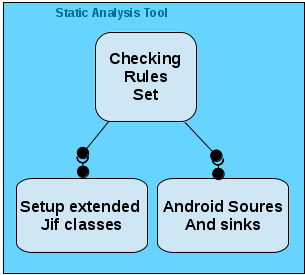
\includegraphics[width=4.6cm]{desing2-inside.png}
	\end{center}
	\caption{Static Analisys Tool Diagrama interno. Ilustra la composición interna
	de la herramienta propuesta para el análisis estático de aplicaciones Android.}
	\label{fig:desing1-in}
\end{figure}

\begin{figure}[t!]
	\begin{center}
	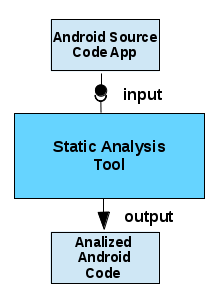
\includegraphics[width=3.5cm]{desing1-2.png}
	\end{center}
	\caption{Static Analisys Tool. Ilustra el input esperado por la herramienta, y
	el resultado devuelto.}
	\label{fig:desing1}
\end{figure} 

Luego, la estrategia de evaluación, consiste en verificar si la herramienta
implementada identifica pérdida de información mediante detección de flujos
implícitos. Esto debido a que, como se menciona en la descripción del problema,
parte importante de las propuestas para detección de fuga de información en
aplicaciones Android, hacen data-flow analysis aplicando técnicas de análisis
tainting, y en contraste con las técnicas de análisis de flujo de información,
las técnicas de análisis tainting no necesariamente consideran flujos
implícitos. Por tanto, al estar basada en JIF, cuyo enfoque de análisis es
precisamente flujo de información, se esperaría que la herramienta planteada
esté en capacidad de reconocer flujos implícitos.

% Se esperaría que: al realizar análisis de flujo de información aplicando
% técnicas Security-Typing, la herramienta propuesta, esté en capacidad de
% reconocer flujos implícitos.\newline
% Más específicamente, se puede tomar el conjunto de aplicaciones utilizadas como
% casos de prueba para la detección de flujos implícitos en
% DroidBench\cite{DroidBenchBenchmarks}, el benchmark de Flowdroid, y analizarlas
% con la herramienta propuesta.\newline

Más específicamente, se puede partir de DroidBench\cite{DroidBenchBenchmarks},
el benchmark de Flowdroid[\ref{FlowDroid-Tool}], tomar el conjunto de
aplicaciones con que prueban la detección de flujos implícitos, y analizarlas
con la herramienta propuesta.\newline
Finalmente estos resultados serían
comparados con los obtenidos mediante otras herramientas para análisis de fuga
de información en aplicaciones Android.\newline

En este orden de ideas, la evaluación de la herramienta propuesta está enfocada
en: medir recall frente a la detección de flujos implícitos, es decir, medir que
no genere falsos negativos ante la existencia de fugas de información,
provenientes de flujos implícitos.\newline

Por último, cabe anotar que aunque la presente propuesta está centrada en
verificar políticas de confidencialidad, en caso de contar con el tiempo
prudente, sería interesante analizar políticas adicionales como por ejemplo,
integridad y declasificación, pues estas son verificables mediante el modelo de
evaluación de JIF, modelo del que parte la herramienta de evaluación planteada.





















